% Generated by code/needham.py -- do not edit by hand.
\definecolor{qocA}{rgb}{0.00,0.45,0.70}
\definecolor{qocB}{rgb}{0.90,0.60,0.00}
\definecolor{qocC}{rgb}{0.00,0.62,0.45}
\definecolor{qocD}{rgb}{0.80,0.40,0.00}
\definecolor{qocE}{rgb}{0.80,0.60,0.70}
\definecolor{qocF}{rgb}{0.35,0.70,0.90}
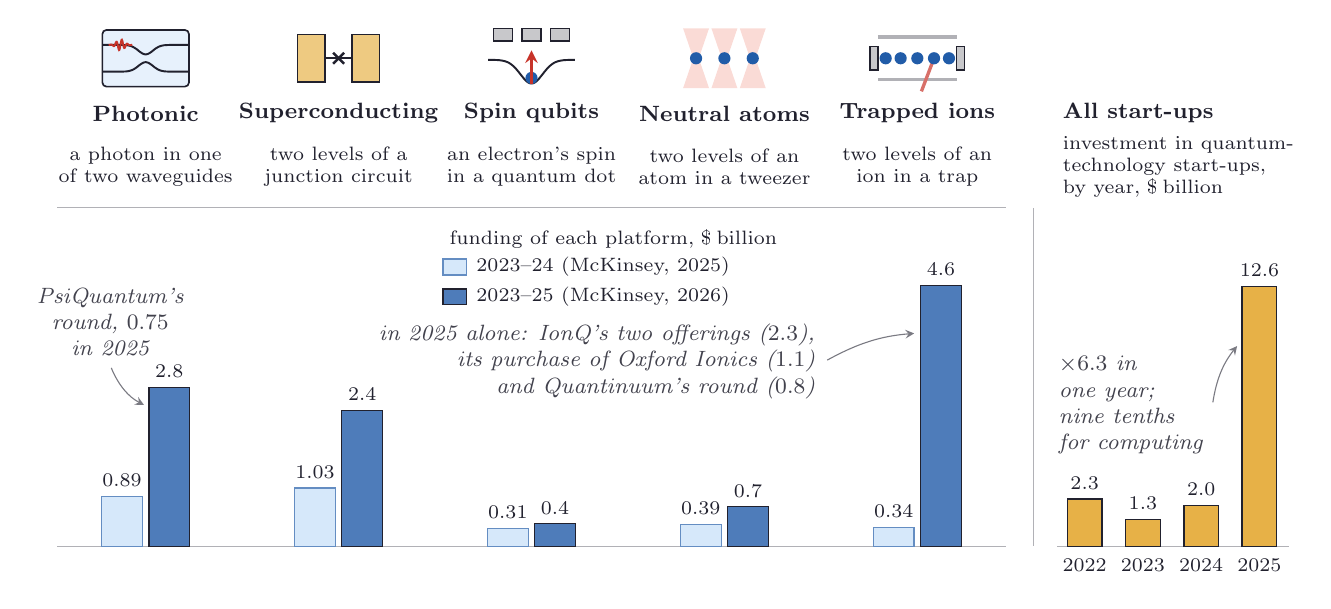
\begin{tikzpicture}[ink/.style={line width=0.9pt, ndInk}, faint/.style={line width=0.4pt, ndInk!35}, dashedink/.style={line width=0.5pt, ndInk!55, dash pattern=on 2.5pt off 2pt}, vec/.style={->, >=stealth, line width=1.2pt}, note/.style={font=\footnotesize\itshape, text=ndInk!85, align=center}, pointer/.style={->, >=stealth, line width=0.4pt, ndInk!60, shorten >=2pt, shorten <=1pt}, dot/.style={circle, fill=ndInk, inner sep=0pt, minimum size=3.4pt}, wash/.style={fill=ndSky, fill opacity=0.55}, every node/.style={text=ndInk}]
\definecolor{ndInk}{rgb}{0.13,0.13,0.18}
\definecolor{ndPaper}{rgb}{0.99,0.96,0.88}
\definecolor{ndSky}{rgb}{0.84,0.91,0.98}
\definecolor{ndRose}{rgb}{0.98,0.86,0.84}
\definecolor{ndBlue}{rgb}{0.13,0.36,0.66}
\definecolor{ndRed}{rgb}{0.78,0.20,0.16}
\definecolor{ndGold}{rgb}{0.88,0.62,0.10}
\definecolor{ndGreen}{rgb}{0.18,0.52,0.30}
\filldraw[fill=ndSky!60, draw=ndInk, line width=0.6pt, rounded corners=1.5pt] (0.675,5.840) rectangle (1.775,6.560);
\draw[ndInk, line width=0.7pt] (0.675,6.370) -- (0.689,6.370) -- (0.703,6.370) -- (0.717,6.370) -- (0.731,6.370) -- (0.745,6.370) -- (0.759,6.370) -- (0.772,6.370) -- (0.786,6.370) -- (0.800,6.370) -- (0.814,6.370) -- (0.828,6.370) -- (0.842,6.370) -- (0.856,6.370) -- (0.870,6.370) -- (0.884,6.370) -- (0.898,6.370) -- (0.912,6.370) -- (0.926,6.369) -- (0.940,6.369) -- (0.953,6.368) -- (0.967,6.368) -- (0.981,6.366) -- (0.995,6.365) -- (1.009,6.362) -- (1.023,6.359) -- (1.037,6.355) -- (1.051,6.350) -- (1.065,6.344) -- (1.079,6.336) -- (1.093,6.327) -- (1.107,6.318) -- (1.121,6.307) -- (1.134,6.296) -- (1.148,6.285) -- (1.162,6.275) -- (1.176,6.266) -- (1.190,6.258) -- (1.204,6.253) -- (1.218,6.250) -- (1.232,6.250) -- (1.246,6.253) -- (1.260,6.258) -- (1.274,6.266) -- (1.288,6.275) -- (1.302,6.285) -- (1.316,6.296) -- (1.329,6.307) -- (1.343,6.318) -- (1.357,6.327) -- (1.371,6.336) -- (1.385,6.344) -- (1.399,6.350) -- (1.413,6.355) -- (1.427,6.359) -- (1.441,6.362) -- (1.455,6.365) -- (1.469,6.366) -- (1.483,6.368) -- (1.497,6.368) -- (1.510,6.369) -- (1.524,6.369) -- (1.538,6.370) -- (1.552,6.370) -- (1.566,6.370) -- (1.580,6.370) -- (1.594,6.370) -- (1.608,6.370) -- (1.622,6.370) -- (1.636,6.370) -- (1.650,6.370) -- (1.664,6.370) -- (1.678,6.370) -- (1.691,6.370) -- (1.705,6.370) -- (1.719,6.370) -- (1.733,6.370) -- (1.747,6.370) -- (1.761,6.370) -- (1.775,6.370);
\draw[ndInk, line width=0.7pt] (0.675,6.030) -- (0.689,6.030) -- (0.703,6.030) -- (0.717,6.030) -- (0.731,6.030) -- (0.745,6.030) -- (0.759,6.030) -- (0.772,6.030) -- (0.786,6.030) -- (0.800,6.030) -- (0.814,6.030) -- (0.828,6.030) -- (0.842,6.030) -- (0.856,6.030) -- (0.870,6.030) -- (0.884,6.030) -- (0.898,6.030) -- (0.912,6.030) -- (0.926,6.031) -- (0.940,6.031) -- (0.953,6.032) -- (0.967,6.032) -- (0.981,6.034) -- (0.995,6.035) -- (1.009,6.038) -- (1.023,6.041) -- (1.037,6.045) -- (1.051,6.050) -- (1.065,6.056) -- (1.079,6.064) -- (1.093,6.073) -- (1.107,6.082) -- (1.121,6.093) -- (1.134,6.104) -- (1.148,6.115) -- (1.162,6.125) -- (1.176,6.134) -- (1.190,6.142) -- (1.204,6.147) -- (1.218,6.150) -- (1.232,6.150) -- (1.246,6.147) -- (1.260,6.142) -- (1.274,6.134) -- (1.288,6.125) -- (1.302,6.115) -- (1.316,6.104) -- (1.329,6.093) -- (1.343,6.082) -- (1.357,6.073) -- (1.371,6.064) -- (1.385,6.056) -- (1.399,6.050) -- (1.413,6.045) -- (1.427,6.041) -- (1.441,6.038) -- (1.455,6.035) -- (1.469,6.034) -- (1.483,6.032) -- (1.497,6.032) -- (1.510,6.031) -- (1.524,6.031) -- (1.538,6.030) -- (1.552,6.030) -- (1.566,6.030) -- (1.580,6.030) -- (1.594,6.030) -- (1.608,6.030) -- (1.622,6.030) -- (1.636,6.030) -- (1.650,6.030) -- (1.664,6.030) -- (1.678,6.030) -- (1.691,6.030) -- (1.705,6.030) -- (1.719,6.030) -- (1.733,6.030) -- (1.747,6.030) -- (1.761,6.030) -- (1.775,6.030);
\draw[ndRed, line width=0.7pt] (0.755,6.369) -- (0.760,6.370) -- (0.765,6.370) -- (0.770,6.371) -- (0.775,6.372) -- (0.780,6.373) -- (0.786,6.374) -- (0.791,6.374) -- (0.796,6.372) -- (0.801,6.369) -- (0.806,6.365) -- (0.811,6.360) -- (0.816,6.356) -- (0.821,6.354) -- (0.826,6.356) -- (0.831,6.362) -- (0.836,6.373) -- (0.841,6.387) -- (0.847,6.400) -- (0.852,6.409) -- (0.857,6.410) -- (0.862,6.402) -- (0.867,6.384) -- (0.872,6.360) -- (0.877,6.335) -- (0.882,6.314) -- (0.887,6.304) -- (0.892,6.308) -- (0.897,6.326) -- (0.902,6.354) -- (0.908,6.386) -- (0.913,6.414) -- (0.918,6.432) -- (0.923,6.436) -- (0.928,6.426) -- (0.933,6.405) -- (0.938,6.380) -- (0.943,6.356) -- (0.948,6.338) -- (0.953,6.330) -- (0.958,6.331) -- (0.963,6.340) -- (0.969,6.353) -- (0.974,6.367) -- (0.979,6.378) -- (0.984,6.384) -- (0.989,6.386) -- (0.994,6.384) -- (0.999,6.380) -- (1.004,6.375) -- (1.009,6.371) -- (1.014,6.368) -- (1.019,6.366) -- (1.024,6.366) -- (1.030,6.367) -- (1.035,6.368) -- (1.040,6.369) -- (1.045,6.370) -- (1.050,6.370) -- (1.055,6.371);
\node[font=\footnotesize\bfseries] at (1.225,5.500) {Photonic};
\node[font=\scriptsize, align=center] at (1.225,4.820) {a photon in one\\ of two waveguides};
\filldraw[fill=ndGold!55, draw=ndInk, line width=0.6pt] (3.505,5.900) rectangle (3.155,6.500);
\filldraw[fill=ndGold!55, draw=ndInk, line width=0.6pt] (3.845,5.900) rectangle (4.195,6.500);
\draw[ndInk, line width=0.7pt] (3.505,6.200) -- (3.845,6.200);
\draw[ndInk, line width=0.9pt] (3.605,6.130) -- (3.745,6.270) (3.605,6.270) -- (3.745,6.130);
\node[font=\footnotesize\bfseries] at (3.675,5.500) {Superconducting};
\node[font=\scriptsize, align=center] at (3.675,4.820) {two levels of a\\ junction circuit};
\filldraw[fill=ndInk!25, draw=ndInk, line width=0.5pt] (5.645,6.420) rectangle (5.885,6.580);
\filldraw[fill=ndInk!25, draw=ndInk, line width=0.5pt] (6.005,6.420) rectangle (6.245,6.580);
\filldraw[fill=ndInk!25, draw=ndInk, line width=0.5pt] (6.365,6.420) rectangle (6.605,6.580);
\draw[ndInk, line width=0.7pt] (5.575,6.180) -- (5.589,6.180) -- (5.603,6.180) -- (5.617,6.180) -- (5.631,6.179) -- (5.645,6.179) -- (5.659,6.179) -- (5.672,6.178) -- (5.686,6.178) -- (5.700,6.177) -- (5.714,6.176) -- (5.728,6.174) -- (5.742,6.172) -- (5.756,6.170) -- (5.770,6.167) -- (5.784,6.164) -- (5.798,6.159) -- (5.812,6.154) -- (5.826,6.148) -- (5.840,6.141) -- (5.853,6.133) -- (5.867,6.123) -- (5.881,6.112) -- (5.895,6.100) -- (5.909,6.086) -- (5.923,6.072) -- (5.937,6.056) -- (5.951,6.039) -- (5.965,6.022) -- (5.979,6.004) -- (5.993,5.986) -- (6.007,5.969) -- (6.021,5.952) -- (6.034,5.936) -- (6.048,5.921) -- (6.062,5.908) -- (6.076,5.897) -- (6.090,5.889) -- (6.104,5.883) -- (6.118,5.880) -- (6.132,5.880) -- (6.146,5.883) -- (6.160,5.889) -- (6.174,5.897) -- (6.188,5.908) -- (6.202,5.921) -- (6.216,5.936) -- (6.229,5.952) -- (6.243,5.969) -- (6.257,5.986) -- (6.271,6.004) -- (6.285,6.022) -- (6.299,6.039) -- (6.313,6.056) -- (6.327,6.072) -- (6.341,6.086) -- (6.355,6.100) -- (6.369,6.112) -- (6.383,6.123) -- (6.397,6.133) -- (6.410,6.141) -- (6.424,6.148) -- (6.438,6.154) -- (6.452,6.159) -- (6.466,6.164) -- (6.480,6.167) -- (6.494,6.170) -- (6.508,6.172) -- (6.522,6.174) -- (6.536,6.176) -- (6.550,6.177) -- (6.564,6.178) -- (6.578,6.178) -- (6.591,6.179) -- (6.605,6.179) -- (6.619,6.179) -- (6.633,6.180) -- (6.647,6.180) -- (6.661,6.180) -- (6.675,6.180);
\fill[ndBlue] (6.125,5.950) circle (2.2pt);
\draw[->, >=stealth, ndRed, line width=1.0pt] (6.125,5.870) -- (6.125,6.300);
\node[font=\footnotesize\bfseries] at (6.125,5.500) {Spin qubits};
\node[font=\scriptsize, align=center] at (6.125,4.820) {an electron's spin\\ in a quantum dot};
\fill[ndRose] (8.050,5.820) -- (8.059,5.846) -- (8.068,5.872) -- (8.077,5.899) -- (8.086,5.925) -- (8.095,5.951) -- (8.104,5.977) -- (8.113,6.003) -- (8.122,6.030) -- (8.131,6.056) -- (8.140,6.082) -- (8.149,6.108) -- (8.158,6.134) -- (8.167,6.161) -- (8.176,6.187) -- (8.176,6.213) -- (8.167,6.239) -- (8.158,6.266) -- (8.149,6.292) -- (8.140,6.318) -- (8.131,6.344) -- (8.122,6.370) -- (8.113,6.397) -- (8.104,6.423) -- (8.095,6.449) -- (8.086,6.475) -- (8.077,6.501) -- (8.068,6.528) -- (8.059,6.554) -- (8.050,6.580) -- (8.380,6.580) -- (8.371,6.554) -- (8.362,6.528) -- (8.353,6.501) -- (8.344,6.475) -- (8.335,6.449) -- (8.326,6.423) -- (8.317,6.397) -- (8.308,6.370) -- (8.299,6.344) -- (8.290,6.318) -- (8.281,6.292) -- (8.272,6.266) -- (8.263,6.239) -- (8.254,6.213) -- (8.254,6.187) -- (8.263,6.161) -- (8.272,6.134) -- (8.281,6.108) -- (8.290,6.082) -- (8.299,6.056) -- (8.308,6.030) -- (8.317,6.003) -- (8.326,5.977) -- (8.335,5.951) -- (8.344,5.925) -- (8.353,5.899) -- (8.362,5.872) -- (8.371,5.846) -- (8.380,5.820) -- cycle;
\fill[ndBlue] (8.215,6.200) circle (2.2pt);
\fill[ndRose] (8.410,5.820) -- (8.419,5.846) -- (8.428,5.872) -- (8.437,5.899) -- (8.446,5.925) -- (8.455,5.951) -- (8.464,5.977) -- (8.473,6.003) -- (8.482,6.030) -- (8.491,6.056) -- (8.500,6.082) -- (8.509,6.108) -- (8.518,6.134) -- (8.527,6.161) -- (8.536,6.187) -- (8.536,6.213) -- (8.527,6.239) -- (8.518,6.266) -- (8.509,6.292) -- (8.500,6.318) -- (8.491,6.344) -- (8.482,6.370) -- (8.473,6.397) -- (8.464,6.423) -- (8.455,6.449) -- (8.446,6.475) -- (8.437,6.501) -- (8.428,6.528) -- (8.419,6.554) -- (8.410,6.580) -- (8.740,6.580) -- (8.731,6.554) -- (8.722,6.528) -- (8.713,6.501) -- (8.704,6.475) -- (8.695,6.449) -- (8.686,6.423) -- (8.677,6.397) -- (8.668,6.370) -- (8.659,6.344) -- (8.650,6.318) -- (8.641,6.292) -- (8.632,6.266) -- (8.623,6.239) -- (8.614,6.213) -- (8.614,6.187) -- (8.623,6.161) -- (8.632,6.134) -- (8.641,6.108) -- (8.650,6.082) -- (8.659,6.056) -- (8.668,6.030) -- (8.677,6.003) -- (8.686,5.977) -- (8.695,5.951) -- (8.704,5.925) -- (8.713,5.899) -- (8.722,5.872) -- (8.731,5.846) -- (8.740,5.820) -- cycle;
\fill[ndBlue] (8.575,6.200) circle (2.2pt);
\fill[ndRose] (8.770,5.820) -- (8.779,5.846) -- (8.788,5.872) -- (8.797,5.899) -- (8.806,5.925) -- (8.815,5.951) -- (8.824,5.977) -- (8.833,6.003) -- (8.842,6.030) -- (8.851,6.056) -- (8.860,6.082) -- (8.869,6.108) -- (8.878,6.134) -- (8.887,6.161) -- (8.896,6.187) -- (8.896,6.213) -- (8.887,6.239) -- (8.878,6.266) -- (8.869,6.292) -- (8.860,6.318) -- (8.851,6.344) -- (8.842,6.370) -- (8.833,6.397) -- (8.824,6.423) -- (8.815,6.449) -- (8.806,6.475) -- (8.797,6.501) -- (8.788,6.528) -- (8.779,6.554) -- (8.770,6.580) -- (9.100,6.580) -- (9.091,6.554) -- (9.082,6.528) -- (9.073,6.501) -- (9.064,6.475) -- (9.055,6.449) -- (9.046,6.423) -- (9.037,6.397) -- (9.028,6.370) -- (9.019,6.344) -- (9.010,6.318) -- (9.001,6.292) -- (8.992,6.266) -- (8.983,6.239) -- (8.974,6.213) -- (8.974,6.187) -- (8.983,6.161) -- (8.992,6.134) -- (9.001,6.108) -- (9.010,6.082) -- (9.019,6.056) -- (9.028,6.030) -- (9.037,6.003) -- (9.046,5.977) -- (9.055,5.951) -- (9.064,5.925) -- (9.073,5.899) -- (9.082,5.872) -- (9.091,5.846) -- (9.100,5.820) -- cycle;
\fill[ndBlue] (8.935,6.200) circle (2.2pt);
\node[font=\footnotesize\bfseries] at (8.575,5.500) {Neutral atoms};
\node[font=\scriptsize, align=center] at (8.575,4.820) {two levels of an\\ atom in a tweezer};
\draw[faint, line width=1.4pt] (10.525,5.930) -- (11.525,5.930);
\filldraw[fill=ndInk!25, draw=ndInk, line width=0.5pt] (10.525,6.050) rectangle (10.425,6.350);
\draw[faint, line width=1.4pt] (10.525,6.470) -- (11.525,6.470);
\filldraw[fill=ndInk!25, draw=ndInk, line width=0.5pt] (11.525,6.050) rectangle (11.625,6.350);
\draw[ndRed!70, line width=1.2pt] (11.077,5.780) -- (11.237,6.200);
\fill[ndBlue] (10.623,6.200) circle (2.2pt);
\fill[ndBlue] (10.813,6.200) circle (2.2pt);
\fill[ndBlue] (11.025,6.200) circle (2.2pt);
\fill[ndBlue] (11.237,6.200) circle (2.2pt);
\fill[ndBlue] (11.427,6.200) circle (2.2pt);
\node[font=\footnotesize\bfseries] at (11.025,5.500) {Trapped ions};
\node[font=\scriptsize, align=center] at (11.025,4.820) {two levels of an\\ ion in a trap};
\draw[faint] (0.1,4.3) -- (12.150,4.3);
\draw[faint] (0.1,0) -- (12.150,0);
\filldraw[fill=ndSky, draw=ndBlue!70, line width=0.5pt] (0.665,0) rectangle (1.185,0.638);
\node[font=\scriptsize, anchor=south] at (0.925,0.638) {0.89};
\filldraw[fill=ndBlue!80, draw=ndInk, line width=0.5pt] (1.265,0) rectangle (1.785,2.016);
\node[font=\scriptsize, anchor=south] at (1.525,2.016) {2.8};
\filldraw[fill=ndSky, draw=ndBlue!70, line width=0.5pt] (3.115,0) rectangle (3.635,0.744);
\node[font=\scriptsize, anchor=south] at (3.375,0.744) {1.03};
\filldraw[fill=ndBlue!80, draw=ndInk, line width=0.5pt] (3.715,0) rectangle (4.235,1.728);
\node[font=\scriptsize, anchor=south] at (3.975,1.728) {2.4};
\filldraw[fill=ndSky, draw=ndBlue!70, line width=0.5pt] (5.565,0) rectangle (6.085,0.225);
\node[font=\scriptsize, anchor=south] at (5.825,0.225) {0.31};
\filldraw[fill=ndBlue!80, draw=ndInk, line width=0.5pt] (6.165,0) rectangle (6.685,0.288);
\node[font=\scriptsize, anchor=south] at (6.425,0.288) {0.4};
\filldraw[fill=ndSky, draw=ndBlue!70, line width=0.5pt] (8.015,0) rectangle (8.535,0.278);
\node[font=\scriptsize, anchor=south] at (8.275,0.278) {0.39};
\filldraw[fill=ndBlue!80, draw=ndInk, line width=0.5pt] (8.615,0) rectangle (9.135,0.504);
\node[font=\scriptsize, anchor=south] at (8.875,0.504) {0.7};
\filldraw[fill=ndSky, draw=ndBlue!70, line width=0.5pt] (10.465,0) rectangle (10.985,0.244);
\node[font=\scriptsize, anchor=south] at (10.725,0.244) {0.34};
\filldraw[fill=ndBlue!80, draw=ndInk, line width=0.5pt] (11.065,0) rectangle (11.585,3.312);
\node[font=\scriptsize, anchor=south] at (11.325,3.312) {4.6};
\filldraw[fill=ndSky, draw=ndBlue!70, line width=0.5pt] (5.000,3.450) rectangle ++(0.3,0.2) node[right, font=\scriptsize, text=ndInk, yshift=-0.1cm] {2023--24 (McKinsey, 2025)};
\filldraw[fill=ndBlue!80, draw=ndInk, line width=0.5pt] (5.000,3.070) rectangle ++(0.3,0.2) node[right, font=\scriptsize, text=ndInk, yshift=-0.1cm] {2023--25 (McKinsey, 2026)};
\node[font=\scriptsize, anchor=west] at (4.960,3.900) {funding of each platform, \$\,billion};
\node[note, anchor=east, align=right] (ion) at (9.850,2.350) {in 2025 alone: IonQ's two offerings ($2.3$),\\ its purchase of Oxford Ionics ($1.1$)\\ and Quantinuum's round ($0.8$)};
\draw[pointer] (ion.east) to[bend left=12] (11.055,2.712);
\node[note, anchor=south] (ps) at (0.775,2.300) {PsiQuantum's\\ round, $0.75$\\ in 2025};
\draw[pointer] (ps.south) to[bend right=20] (1.265,1.766);
\draw[faint] (12.500,4.3) -- (12.500,0);
\node[font=\footnotesize\bfseries, anchor=west] at (12.750,5.500) {All start-ups};
\node[font=\scriptsize, align=left, anchor=west] at (12.750,4.820) {investment in quantum-\\technology start-ups,\\ by year, \$\,billion};
\draw[faint] (12.800,0) -- (15.750,0);
\filldraw[fill=ndGold!80, draw=ndInk, line width=0.5pt] (12.930,0) rectangle (13.370,0.602);
\node[font=\scriptsize, anchor=south] at (13.150,0.602) {2.3};
\node[font=\scriptsize, anchor=north] at (13.150,-0.04) {2022};
\filldraw[fill=ndGold!80, draw=ndInk, line width=0.5pt] (13.670,0) rectangle (14.110,0.340);
\node[font=\scriptsize, anchor=south] at (13.890,0.340) {1.3};
\node[font=\scriptsize, anchor=north] at (13.890,-0.04) {2023};
\filldraw[fill=ndGold!80, draw=ndInk, line width=0.5pt] (14.410,0) rectangle (14.850,0.524);
\node[font=\scriptsize, anchor=south] at (14.630,0.524) {2.0};
\node[font=\scriptsize, anchor=north] at (14.630,-0.04) {2024};
\filldraw[fill=ndGold!80, draw=ndInk, line width=0.5pt] (15.150,0) rectangle (15.590,3.300);
\node[font=\scriptsize, anchor=south] at (15.370,3.300) {12.6};
\node[font=\scriptsize, anchor=north] at (15.370,-0.04) {2025};
\node[note, anchor=south west, align=left] (x6) at (12.700,1.050) {$\times6.3$ in\\ one year;\\ nine tenths\\ for computing};
\draw[pointer] (x6.east) to[bend left=15] (15.130,2.600);
\end{tikzpicture}
